\documentclass[10pt, twoside]{report}
\usepackage[utf8]{inputenc}
\usepackage[english]{babel}
\usepackage{helvet}
\renewcommand{\familydefault}{\sfdefault}
\usepackage{enumitem}
\usepackage{amsmath}
\usepackage[makeroom]{cancel}
%%%% math color boxç
\usepackage{xcolor}
\usepackage{soul}
\newcommand{\mathcolorbox}[2]{\colorbox{#1}{$\displaystyle #2$}}
\newcommand{\hlfancy}[2]{\sethlcolor{#1}\hl{#2}}
%%%% end math color box
\usepackage{tikz}
\usetikzlibrary{quotes,angles}
\usetikzlibrary{positioning,shapes,shadows,arrows}
\usepackage{lastpage}
\usepackage{listings}
\usepackage{listingsutf8}
\usepackage{booktabs}
\usepackage[acronym]{glossaries}
\usepackage{smartdiagram}
\usesmartdiagramlibrary{additions}
\usepackage{imakeidx}
\makeindex[columns=3, title=Index]
\usepackage{wrapfig}
\usepackage{amsmath} 
\usepackage{amssymb}
\usepackage{amsfonts}
\usepackage{float}
\usepackage[edges]{forest}
\usetikzlibrary{arrows.meta}
\usepackage{rotating}
\usepackage{etoolbox}
\usepackage{courier}
\usepackage{lmodern}
%shade begin
\usepackage{framed}
\usepackage[most]{tcolorbox}
\usepackage{xcolor}
\colorlet{shadecolor}{blue!10}
%shade end
\usepackage{makeidx}
\usepackage{caption}
\usepackage{tabularx}
\usepackage{subcaption}
\usepackage{lscape}
\usepackage{chngcntr}
\usepackage{csquotes}
\usepackage{graphicx}
\usepackage{mathtools}
\usepackage{multicol,caption}
\usepackage{multirow}
\usepackage{lipsum}
\usepackage{titlesec}
\usepackage{tocloft}
\usepackage[T1]{fontenc}
\usepackage{titlesec}
\usepackage{url}
% \usepackage[framed,numbered,autolinebreaks,useliterate]{mcode}
\raggedbottom
\setlength{\parindent}{0pt}
\setlength{\parskip}{7pt}
\usepackage{geometry}
\geometry{
    a4paper, 
    total={170mm,247mm}, 
    left=20mm, 
    top=30mm
}
\usepackage{hyperref}
\hypersetup{
    colorlinks=true,
    linkcolor=blue,
    filecolor=magenta,      
    urlcolor=cyan,}
\usepackage{placeins} %FloatBarrier
\usepackage[nottoc]{tocbibind}
\usepackage[backend=biber,style=numeric,sorting=none]{biblatex}
\usepackage{fancyhdr}

\usepackage{chemfig}
\usepackage{graphicx}
\usepackage[version=3]{mhchem}

\setlength{\floatsep}{15pt}

% Unidades tiempo
\newcommand{\second}{\mathrm{s}}
\newcommand{\hour}{\mathrm{h}}
\newcommand{\minute}{\mathrm{min}}
% Unidades temperatura
\newcommand{\celsius}{\mathrm{^{\circ} C}}
\newcommand{\fahrenheit}{\mathrm{^{\circ} F}}
\newcommand{\kelvin}{\mathrm{K}}
% Unidades distancia
\newcommand{\meter}{\mathrm{m}}
\newcommand{\cmeter}{\mathrm{cm}}
\newcommand{\mmeter}{\mathrm{mm}}
% Unidades area
\newcommand{\sqmeter}{\mathrm{m^2}}
% Unidades volumen
\newcommand{\cbmeter}{\mathrm{m^3}}
\newcommand{\liter}{\mathrm{L}}
\newcommand{\milliliter}{\mathrm{mL}}
\newcommand{\mliter}{\mathrm{mL}}
% Unidades energia
\newcommand{\joule}{\mathrm{J}}
\newcommand{\watt}{\mathrm{W}}
% Unidades de masa y cantidad\newcommand{\gram}{\mathrm{g}}
\newcommand{\kg}{\mathrm{kg}}
\newcommand{\mol}{\mathrm{mol}}
% Unidades presion
\newcommand{\atm}{\mathrm{atm}}
\newcommand{\pascal}{\mathrm{Pa}}
\newcommand{\mpascal}{\mathrm{MPa}}
\newcommand{\presbar}{\mathrm{bar}}
\newcommand{\presmbar}{\mathrm{mbar}}
\newcommand{\mmhg}{\mathrm{mmHg}}
% Unidades eléctricas
\newcommand{\hertz}{\mathrm{Hz}}
\newcommand{\coulomb}{\mathrm{C}}
\newcommand{\ampere}{\mathrm{A}}
\newcommand{\volt}{\mathrm{V}}
\newcommand{\ohm}{\mathrm{\Omega}}
\newcommand{\faraday}{\mathrm{F}}
% Unidades de fuerza
\newcommand{\newton}{\mathrm{N}}
% Múltiplos
\newcommand{\giga}{\mathrm{G}}
\newcommand{\mega}{\mathrm{M}}
\newcommand{\kilo}{\mathrm{k}}
\newcommand{\centi}{\mathrm{c}}
\newcommand{\milli}{\mathrm{m}}
\newcommand{\micro}{\mathrm{\mu}}
\newcommand{\nano}{\mathrm{n}}

% Renewcommands
\captionsetup{labelfont=bf}
\captionsetup{labelsep=space}
% Newcommands
\newcommand{\dd}{\mathrm{d}}
\newcommand{\wt}{\mathrm{wt{\mkern-4mu}\%}}
\newcommand{\vol}{\mathrm{vol{\mkern-4mu}\%}}
\newcommand*{\intentionalblankpage}{%
\vspace*{\fill}
{\centering Esta página ha sido intencionalmente dejada en blanco\par}
\vspace{\fill}}
\makeatletter
\renewcommand*{\cleardoublepage}{\clearpage\if@twoside \ifodd\c@page\else
\blankpage
\thispagestyle{empty}
\clearpage
\if@twocolumn\hbox{}\newpage\fi\fi\fi}

\renewcommand{\cftsecleader}{\cftdotfill{\cftdotsep}}
\titleformat{\section}{\normalfont\fontsize{15}{15}\bfseries}{\thesection}{1em}{}
\setlength{\columnsep}{30pt}

\newcommand\textequal{\rule[.5ex]{6pt}{0.4pt}\llap{\rule[.9ex]{6pt}{0.4pt}}}

\usepackage{makecell}
\usepackage{siunitx}
\usepackage{tikz}   %TikZ is required for this to work.  Make sure this exists before the next line

% \usepackage{3dplot} %requires 3dplot.sty to be in same directory, or in your LaTeX installation

%\usepackage[active,tightpage]{preview}  %generates a tightly fitting border around the work
%\PreviewEnvironment{tikzpicture}
%\setlength\PreviewBorder{2mm}

%\DeclareCaptionFormat{myformat}{#1#2#3\hrulefill}
%\captionsetup[figure]{format=myformat}
\titleformat{\chapter}[block]
  {\normalfont\huge\bfseries}{\thechapter.}{1em}{\LARGE}
\titlespacing*{\chapter}{0pt}{-19pt}{0pt}
\patchcmd{\chapter}{\thispagestyle{plain}}{\thispagestyle{fancy}}{}{}

%%Pàg següent capítol en mateixa pàgina:
\patchcmd{\chapter}{\if@openright\cleardoublepage\else\clearpage\fi}{}{}{}

\newenvironment{Figure}
  {\par\medskip\noindent\minipage{\linewidth}}
  {\endminipage\par\medskip}
\title{Mecànica de vol - GrETA}
\author{Irene Simó}
\date{QT 2021-22}
\pagestyle{fancy}
\lhead{Immelmann turn: A flight mechanics study - Irene Simó} 
\rhead{Page \thepage\ of \pageref*{LastPage}}
\cfoot{}

\begin{document}\thispagestyle{empty} 
	\begin{center}
	\LARGE \textbf{Immelmann turn}\\
	\Large A flight mechanics study\\
		\normalsize
	\begin{tabularx}{\textwidth}{l r}
		Irene Simó Muñoz & Prof: Àlex Ferrer Farré\\
		irene.munoz@estudiantat.upc.edu & Fall 2021
	\end{tabularx}

	\hrule
	\end{center}
	This brief project aims to take a look at the flight mechanics involved in the Immenlman turn maneuver while analysing its performance in a realistic context. \\ For this, a first set of computations have been performed in order to obtain the models of the physic phenomena occurring, and a later sutdy with aircraft values has been carried out to evaluate the previously obtained results.\\
	All the coding has been done with \textsc{matlab}\footnote{MATrix LABoratory, language developed by The MathWorks Inc.} version R2021b (September 2021). The git repository of this project, including the \LaTeX files, can be found in \hyperlink{https://github.com/isimo00/immelmann-turn}{this link}.\\
	This project has been developed for course 22027-Mecànica del vol in the Grau en Enginyeria en Tecnologies Aeroespacials degree, Universitat Politècnica de Catalunya, during fall 2021.
	
	\begin{multicols}{2}
	\vspace*{-2cm}
	\tableofcontents
	\section*{Introduction}
	\addcontentsline{toc}{section}{Introduction}
	\vspace{-0.5cm}
The Immelmann turn, named after German World War I flying ace Max Immelmann, is an an  aerobatic maneuver that results in level-flight of the aircraft in the opposite direction and higher altitude.


\includegraphics[width=\linewidth]{figures/immelmann-overview}
\captionof{figure}{Immelmann turn overview}
\vspace*{0.5cm}

The aircraft initiates this maneuver in straight levelled flight, and describes an upwards semicircle contained in its symmetry plane. This increases the flight altitude while changing the trajectory's to the original's opposite direction and leaves the plane turned upside down. It then rolls while still flying in a straigth line, and returns to the initial condition of levelled flight.\\

This maneuver can be performed for various velocities and radius, but there are some dependencies and limitiations to be taken into account, such as the maximum deflections or forces the control surfaces can provide or support, respectively. 

The higher the velocity is, the bigger the radius - this is, the greater the increase of altitude - given that the wing's flaps cannot deflect enough nor can support as much force to reduce the radius as to the same menauver for a lowe velocity.

Note that the centripetal force follows:
\[
	F=\frac{mV^2}{R}
\]
Where \textit{m}, \textit{V} and \textit{R} are the aircraft's mass (in kg), velocity (in m/s) and radius (in m) respectively. \\

The only angles affected are gamma $\gamma$ and mu $\mu$ if performed flawlessly. The former is the angle formed between the \textit{x} axis of the horizontal set and the \textit{x} axis of the wind set, while the latter is the one formed between the \textit{y} axis of the same sets. Note that for the whole maneuver the body set remains consistent with the wind set.\\
Figure \ref{fig:paramEvolution} shows how these change in the different phases of the Immelmann turn\\

	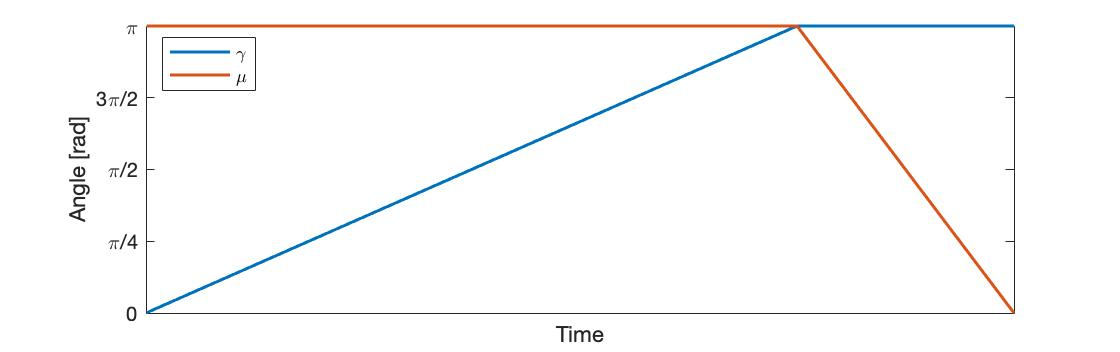
\includegraphics[width=\linewidth]{../matlab/paramEvolution.jpg}
	\captionof{figure}{Angles evolution over time}
	\label{fig:paramEvolution}
	\vspace{0.5cm}

Note that for $\gamma$ the evolution is perfectly defined, as the increment of said angle needs to be positive in order to increase the flight altitude. Conversely, for $\mu$ the pilot could choose to rotate in the opposite direction thus changing $\mu$ from 0 to $-\pi$ instead - note that $\pi$ and $-\pi$ are equivalent -, and the result would be virtually the same.\\
Furthermore, in order to describe a perfect semicircle the angular speed $\dot{\gamma}$ needs to remain constant. This results in the necessary condition of gamma's evolution to be a straight slope. For $\mu$, however, the pilot could also perform the roll at non-constant rotating speed without this having an impact on the maneuver performance. This would be reflected as a curve on mu's temporal evolution, instead of a straight line.


	\section*{Maneouver Computations}
\addcontentsline{toc}{section}{Maneouver Computations}
Let us assume symmetric flight (no lateral aerodynamic force $Q=0$ nor lateral thrust force as $\nu=0$), the thrust generated by the engines is parallel to the \textit{x} wind axis (thus $\epsilon=0$),  and that the maneuver takes place flawlessly, this is in the vertical plane too; $\xi=\dot{\xi}=0$.\\
As the maneuver is a rather short, we will also assume that the fuel consumed i negligible and no mass fraction is lost; $\dot{m}=0$.\\
The motion equations follow:

\begin{equation*}
	\begin{cases}
	T\cos(\epsilon)\cos(\nu) - D -mg\sin\gamma-m\dot{V}=0\\
	T\cos(\epsilon)\sin(\nu) - Q+mg\cos\gamma\sin\mu+mV(\dot{\gamma}\sin\mu-\dot{\Xi}\cos\gamma\cos\mu)=0\\
	-T\sin\epsilon-L+mg\cos\gamma\cos\mu+mV(\dot{\gamma}\cos\mu-\dot{\Xi}\cos\gamma\sin\mu)=0\\
	\dot{x}_e=V\cos\gamma\cos\Xi\\
	\dot{y}_e=V\cos\gamma\sin\Xi\\
	\dot{x}_e=-V\sin\gamma
	\end{cases}
\end{equation*}

And for each of the phases that compose the maneuver, they can be simplified by substituting the flight conditions.

\begin{center}
\begin{tabular}{|l|c|c|c|}\hline
	& $\mu$ & $\gamma=\dot{\gamma}$ & $\xi=\dot{\xi}=\nu=\epsilon=Q$\\ \hline  \hline
	Cruise & 0 & 0 & 0 \\ \hline
	Semicirle & 0 & f(t) & 0 \\ \hline
	Inversion& f(t) & 0 & 0 \\ \hline
\end{tabular}
\end{center}

\subsection*{First phases - cruise}
\addcontentsline{toc}{subsection}{Maneouver Computations}
\begin{equation}
	\begin{cases}
		T - D -m\dot{V}=0\\
		0=0\\
		-L+mg=0\\
		\dot{x}_e=V\\
		\dot{y}_e=0\\
		\dot{x}_e=0
	\end{cases}
\end{equation}
There are three equations and four variables; $\alpha$, $\pi$ and V
Total degrees of freedom are:

\subsection*{Second phase - semicircle}
\addcontentsline{toc}{subsection}{Maneouver Computations}
\begin{equation}
	\begin{cases}
		T - D -mg\sin\gamma-m\dot{V}=0\\
		0=0\\
		-L+mg\cos\gamma+mV\dot{\gamma}=0\\
		\dot{x}_e=V\cos\gamma\\
		\dot{y}_e=0\\
		\dot{z}_e=-V\sin\gamma
	\end{cases}
\label{eq:semicircle}
\end{equation}
There are four equations and four variables: $\alpha$, $\pi$, V and $\gamma$. Timón de profundidad (elevator), palanca de gases (gas control lever or throttle).
Total degrees of freedom are:


\subsection*{Third phase - inversion}
\addcontentsline{toc}{subsection}{Maneouver Computations}
\begin{equation}
	\begin{cases}
		T - D -m\dot{V}=0\\
		mg\sin\mu=0\\
		-L-mg\cos\mu=0\\
		\dot{x}_e=V\\
		\dot{y}_e=0\\
		\dot{z}_e=0
	\end{cases}
\end{equation}
There are three equations and five variables; $\alpha$, $\pi$, V and $\mu$ Ailerons para mu.
Total degrees of freedom are:

\subsection*{Forth phase - cruise}
\addcontentsline{toc}{subsection}{Maneouver Computations}
\begin{equation}
	\begin{cases}
		T - D -m\dot{V}=0\\
		0=0\\
		-L+mg=0\\
		\dot{x}_e=V\\
		\dot{y}_e=0\\
		\dot{z}_e=0
	\end{cases}
\end{equation}
There are three equations and four variables; $\alpha$, $\pi$ and V.
Total degrees of freedom are:	
	\section*{Maneouver study}
\addcontentsline{toc}{section}{Maneouver study}

\subsection{Evolution throughout time}
Evaluate L, D, V, $\gamma$, z, x

Taking the first equation of each of the phases' systems we can operate to integrate the velocity through time. For the most generic case:
\begin{align*}
	0=&T - D -mg\sin\gamma-m\frac{\partial V}{\partial t}\\
	dt =& \frac{m}{T - D -mg\sin\gamma} dV\\
	\int dt= & \int \frac{m}{T - D -mg\sin\gamma} dV
	\intertext{Subsituting drag's definition,}
	= & \int \frac{m}{T - \frac{1}{2}\rho S V^2 (C_{D_0}+kC_L^2) -mg\sin\gamma} dV
\end{align*}


\subsection{Trajectory analysis} 
The three force configurations during the maneuver correspond to the free body diagrams at stages 1, 2 and 3 (see Figure \ref{fig:immelmann-overview}). \vspace{0.5cm}

%\begin{minipage}{\textwidth}
	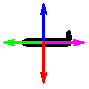
\includegraphics[width=0.3\linewidth]{figures/free-body-1.pdf} \hfill
%	\captionof{subfigure}{Angles evolution over time}
	\label{fig:free-body-1}
		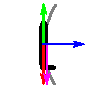
\includegraphics[width=0.3\linewidth]{figures/free-body-2.pdf}\hfill
%	\captionof{subfigure}{Angles evolution over time}
	\label{fig:free-body-2}
		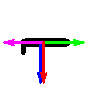
\includegraphics[width=0.3\linewidth]{figures/free-body-3.pdf}
%	\captionof{subfigure}{Angles evolution over time}
	\label{fig:free-body-3}
	\vspace{0.5cm}
%\end{minipage}

Note that at all times the lift behaves as the centripetal force, thus indicating that both the velocity and radius limitations to perform the Immelmann turn are inherent to the wing design and its maximum and minimum lift generation.\\
AS the motion will be circular, the normal and tangential accelerations will follow:
\begin{align*}
	a_n=&\frac{V^2}{R}=V\dot{\gamma}=\dot{\gamma}^2R&a_t=V^2R
\end{align*}
As a result, the radius can be writen as a function of the angle of attack. By operating with the third equation of system number \ref{eq:semicircle}, which is in wind system of reference, very convenient as is also polar system:
\begin{align*}
	L=&m\left(\frac{V^2}{R}+g\cos(\gamma)\right)\\
	\frac{1}{2}\rho S V^2 C_L(\alpha)=&m\left(\frac{V^2}{R}+g\cos(\gamma)\right)\\
	R=&\frac{2mV^2}{2W\cos(\gamma)+\rho S V^2 C_L(\alpha)}
\end{align*}
As the plane must describe a semicircle, the radius must be constant.

Plot x, z with time y despues en plano (ver trayectoria).
We can consider the maneuver coordinates:
\begin{align*}
	\dot{x}_e=&V\cos\gamma&&&	x_e=&Vt\cos\gamma \\
	\dot{y}_e=&0& \rightarrow&&	y_e=&0\\
	\dot{x}_e=&-V\sin\gamma&&&z_e=&-Vt\sin\gamma
\end{align*}

If we take both V (controlled by the gas control lever) and $\gamma$ 
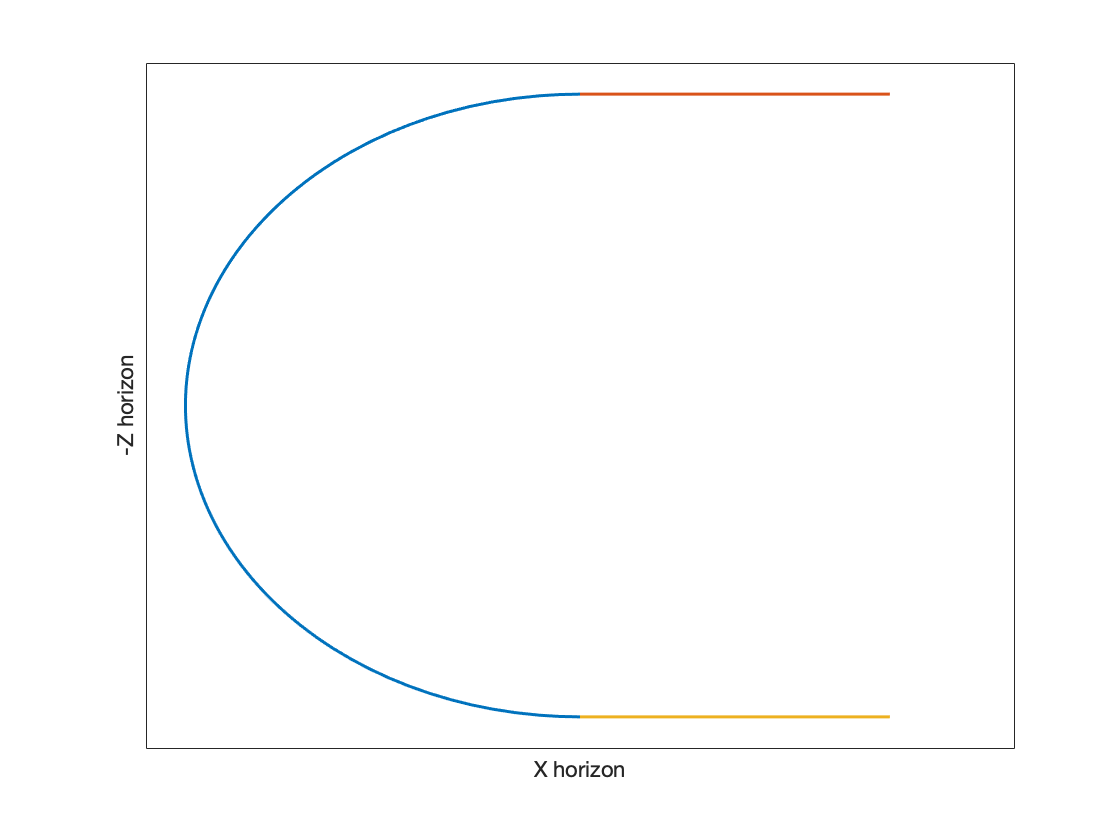
\includegraphics[width=\linewidth]{../matlab/trajectory.png}

	
	\section*{Other data}
	\addcontentsline{toc}{section}{Introduction}
	this is a biblatex test \cite{tierno}
	\end{multicols}\clearpage
\bibliographystyle{plain} % We choose the "plain" reference style
\bibliography{immelmannbib.bib}
\listoffigures
\clearpage
\appendix
\section*{Appendix: Curve fitting}
In order to plot the evolution of both Lift and Drag for each phase, the computated velocity - solved from each respective ODE system - has been fitted from the resultant set of data points into a curve.\\
For this, the native \texttt{polyfit} and \texttt{poly2sym} \textsc{matlab} functions have ben employed. 

To correctly fit a set of points into a curve and avoid overfitting the polynomial (thus dealing with excessive oscillations and Runge's phenomemenon among others), the lienar Least Squares Method (LLS) has been used. The following plots show the square root sum and the norm of the squared regression value for each phase's velocity fit.

\begin{center}
	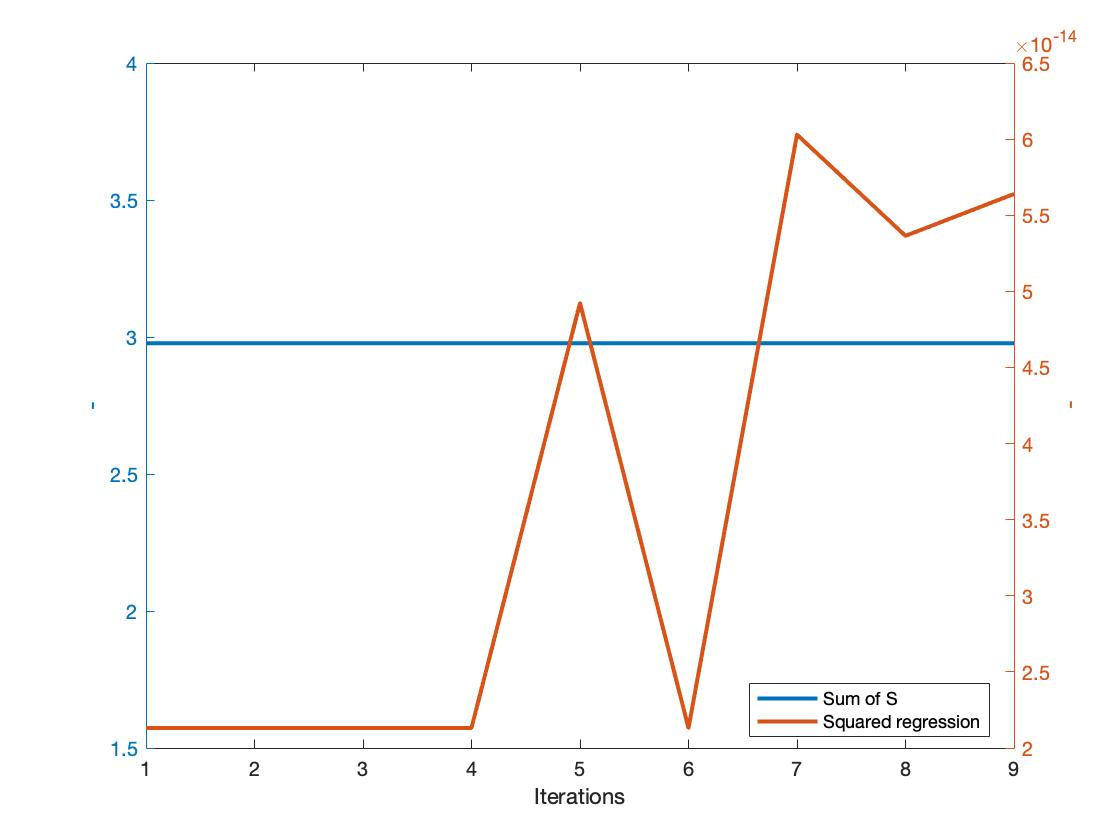
\includegraphics[width=0.45\linewidth]{../matlab/1/1reg.jpg}
	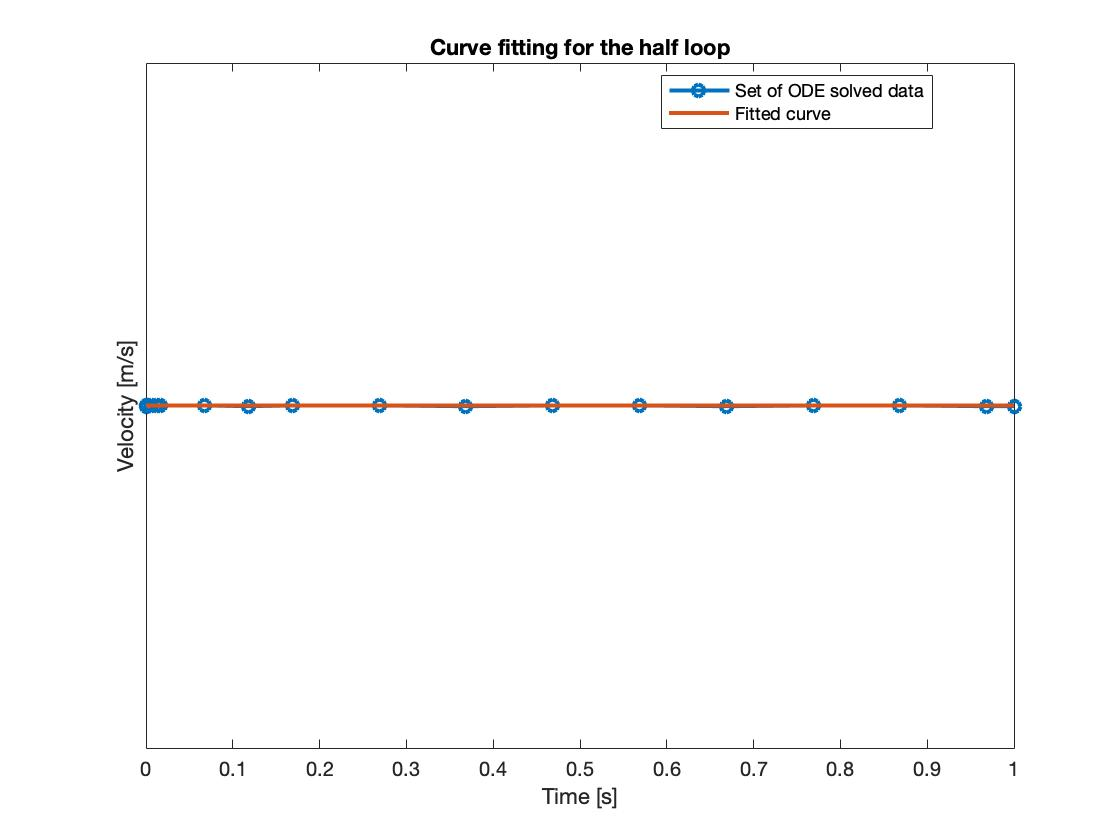
\includegraphics[width=0.45\linewidth]{../matlab/1/1fit.jpg}
	\vspace{0.5cm}
	\captionof{figure}{Lift and drag on the half loop. Own elaboration.}
	\label{fig:1reg}
	\captionof{figure}{Lift and drag on the half loop. Own elaboration.}\vspace{0.25cm}
	\label{fig:1fit}
\end{center}

\begin{center}
	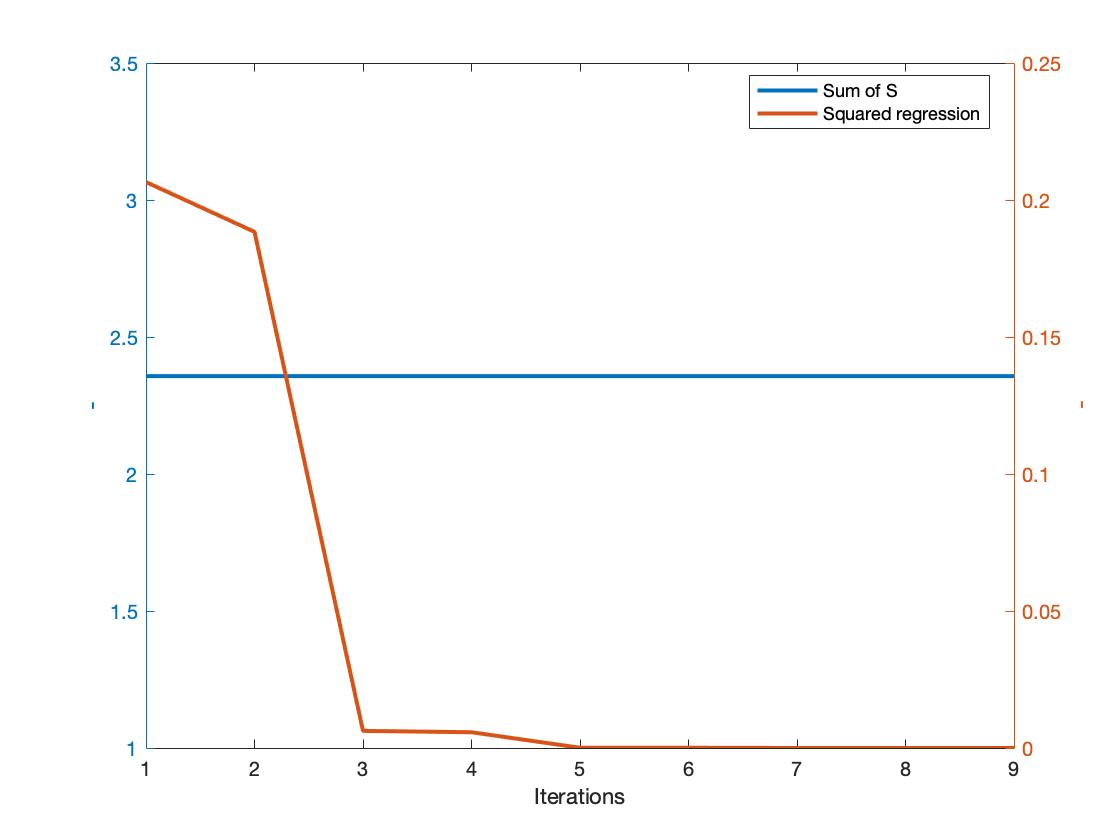
\includegraphics[width=0.45\linewidth]{../matlab/2reg.jpg}
	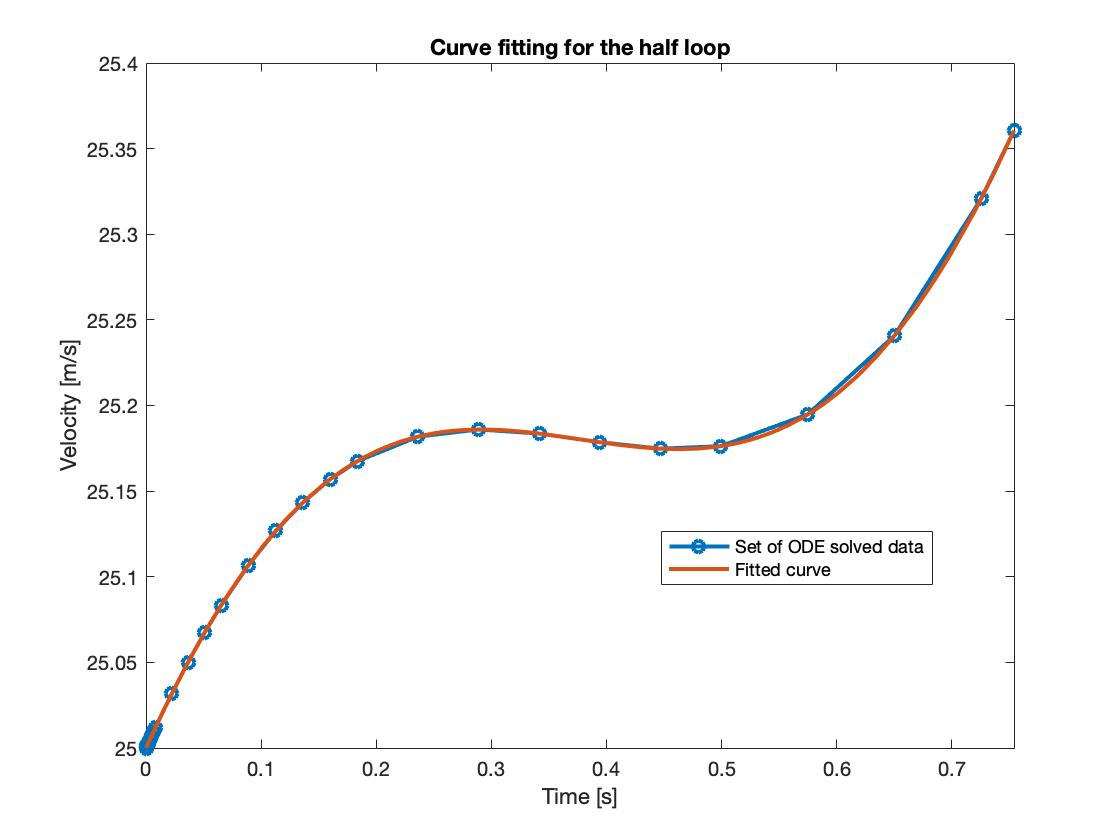
\includegraphics[width=0.45\linewidth]{../matlab/2fit.jpg}
	\vspace{0.5cm}
	\captionof{figure}{Lift and drag on the half loop. Own elaboration.}
	\label{fig:2reg}
	\captionof{figure}{Lift and drag on the half loop. Own elaboration.}\vspace{0.25cm}
	\label{fig:2fit}
\end{center}
\end{document}